\documentclass[11pt,a4paper]{article}
\usepackage[margin=2.5cm]{geometry}
\usepackage{amsmath,amssymb,amsthm,mathtools}
\usepackage{booktabs,graphicx,array,url}
\usepackage[hidelinks,pdftitle={MUG-I v001: Maxwell Mode Geometry and Torsion-Class Carry Activation},pdfauthor={UNNS Research Collective}]{hyperref}
\urlstyle{same}
\setlength{\parindent}{0pt}\setlength{\parskip}{0.55em}
\renewcommand{\arraystretch}{1.25}
\emergencystretch=4em

\newtheorem{theorem}{Theorem}[section]
\newtheorem{proposition}[theorem]{Proposition}
\newtheorem{lemma}[theorem]{Lemma}
\newtheorem{corollary}[theorem]{Corollary}
\theoremstyle{definition}
\newtheorem{definition}[theorem]{Definition}
\theoremstyle{remark}
\newtheorem{remark}[theorem]{Remark}
\newtheorem{example}[theorem]{Example}

\newcommand{\N}{\mathbb N}\newcommand{\Q}{\mathbb Q}\newcommand{\R}{\mathbb R}\newcommand{\Z}{\mathbb Z}
\newcommand{\bE}{\mathbf E}\newcommand{\bB}{\mathbf B}
\DeclareMathOperator{\sqf}{sf}
\DeclareMathOperator{\den}{den}

\title{\bfseries MUG-I v001\\[2pt] Maxwell Mode Geometry and Torsion-Class Carry Activation}
\author{UNNS Research Collective}
\date{Version 001 \quad November 2026}

\begin{document}
\maketitle

\begin{abstract}
\noindent
We lay exact source-free electromagnetic eigenmodes in periodic domains and in an ideal conducting box over the UNNS transition $T_N(x)=x(N+1)^2/N$, $N\mid x$, and over the torsion-class carries of~\cite{TC}, and we separate what is inherited from integer labels from what concerns the fields. On the periodic $3$-torus a mode $m\in\Z^3$ factors as content times primitive direction, $m=g\,u$; every $T_N$ preserves $u$ and multiplies $g$ by $r_N=(N+1)^2/N$. The spectral class of the mode in $\R_{>0}/\Q_{>0}$ is $[\sqrt\sigma]$, $\sigma=\sqf(u\cdot u)$, and the classes that occur are exactly the squarefree $\sigma\not\equiv7\pmod 8$ (Legendre). The transport $\bE'(\mathbf r,t)=\bE(\alpha\mathbf r,\alpha t)$ is an exact Maxwell symmetry that fixes direction, polarization, amplitude and energy and multiplies frequency by $\alpha$; admissibility of a history on a multimode field is the gcd of its support, and the transported field depends on a history only through the product of its multipliers, so no field-level history invariant exists beyond that product. Torsion carries are realized in two ways. Between two cavities of lengths $L_i=L_0/a_i$ they are the rational index maps $c_i$ of~\cite{TC}, and the arithmetic of the layered spectrum is ordinary commensurability. Inside one cavity a carry would be a field-level similarity of the mode lattice; we show that such a similarity with a non-rational ratio does not exist for $D$ odd, in particular on the $3$-torus, exists in $D=2$ exactly for ratios $\sqrt\sigma$ with $\sigma$ a sum of two squares, where it is Gaussian multiplication, and in that case it reproduces the $\sqrt2$ carry layers of~\cite{TC} exactly. All results are verified by an exact suite (12 checks, symbolic Maxwell residuals included). No mode-conversion mechanism is claimed.
\end{abstract}

%% ----------------------------------------------------------------
\section{Scope and the classification rule}
The earlier Maxwell investigation~\cite{MX} established that the dilation $\bE'(\mathbf r,t)=\bE(\alpha_N\mathbf r,\alpha_Nt)$, $\bB'$ likewise, with $\alpha_N=r_N$, maps periodic vacuum waves of harmonic index divisible by $N$ onto those divisible by $(N+1)^2$, and that Maxwell's equations single out no particular $\alpha$. We keep that control: every statement below is placed in one of two columns.
\begin{itemize}
\item \textbf{Label-level:} follows from integer or lattice arithmetic of mode labels and would hold for any family of objects carrying those labels.
\item \textbf{Field-level:} depends on the electromagnetic fields (polarization, boundary conditions, energy, symmetry maps).
\end{itemize}
Throughout, vacuum, $\varepsilon_0,\mu_0$ constant, $c^{-2}=\varepsilon_0\mu_0$, and
\[
\nabla\times\bE=-\partial_t\bB,\qquad \nabla\times\bB=c^{-2}\partial_t\bE,\qquad \nabla\!\cdot\bE=\nabla\!\cdot\bB=0 .
\]
The sources of the arithmetic are \cite{AT} (rational completeness, classes $x\Q_{>0}$) and \cite{TC} (torsion classes, carry law $\alpha a_in=a_{i+1}c_in$, enabling).

\begin{table}[ht]\centering\small
\begin{tabular}{@{}llp{7.6cm}@{}}
\toprule\textbf{Result}&\textbf{Level}&\textbf{Content}\\\midrule
Prop.~\ref{prop:cd}&label&$m=g\,u$; $T_N$ acts on $g$ only, fixes $u$\\
Thm.~\ref{thm:cls}&label (spectral)&spectral classes $[\sqrt\sigma]$, $\sigma\not\equiv7\ (8)$\\
Thm.~\ref{thm:tr}&field&exact transport; fixes $u$, polarization, energy; frequency $\times\alpha$, action $/\alpha$\\
Prop.~\ref{prop:gcd}&label&multimode admissibility $=$ gcd of support\\
Prop.~\ref{prop:hist}&field&no history invariant beyond $\prod r_{N_i}$\\
Thm.~\ref{thm:cav}&label (spectral)&inter-cavity carries are rational index maps $c_i$\\
Thm.~\ref{thm:sim}&field (symmetry)&intra-cavity carry $=$ lattice similarity: none for $D$ odd; $D=2$ iff $\sigma=a^2+b^2$\\
Prop.~\ref{prop:gauss}&field&Gaussian carry equals the $\sqrt2$ layers of~\cite{TC}\\
Prop.~\ref{prop:box}&field&conducting box: wall conditions kept iff index vector integral\\
\bottomrule\end{tabular}\caption{Results and their level.}\end{table}

%% ----------------------------------------------------------------
\section{Exact mode geometry}
\begin{definition}
The periodic cubic cell of side $L$ has modes $(m,\epsilon)$, $m\in\Z^3\setminus\{0\}$, $\epsilon$ one of the two transverse polarizations, with $\mathbf k=\tfrac{2\pi}{L}m$ and $\omega=c|\mathbf k|=\omega_0|m|$, $\omega_0=2\pi c/L$. For $m=g\,u$ with $g=\gcd(m_1,m_2,m_3)$ the vector $u$ is the \emph{primitive direction} and $g$ the \emph{content}.
\end{definition}

\begin{proposition}[Content and direction]\label{prop:cd}
For $N\ge1$: $r_Nm\in\Z^3$ iff $N\mid g$. In that case $r_Nm=g'u$ with $g'=r_Ng$, so $T_N$ fixes $u$ and acts on $g$ as the UNNS transition. Distinct primitive directions are never connected by any history of $T_N$.
\end{proposition}
\begin{proof}
$\gcd(N,N+1)=1$, so $(N+1)^2m_j/N\in\Z$ iff $N\mid m_j$, for $j=1,2,3$, iff $N\mid g$. The rest is immediate.
\end{proof}
Thus the mode set is $\bigsqcup_u\{g\,u:g\in\N_{>0}\}$, and each ray carries the integer grammar of the UNNS substrate.

\begin{theorem}[Spectral classes of the cubic cavity]\label{thm:cls}
Write $u\cdot u=\sigma t^2$ with $\sigma$ squarefree. The frequency of $(g\,u)$ is $\omega_0\,gt\sqrt\sigma$, so its class in $\R_{>0}/\Q_{>0}$ is $[\sqrt\sigma]$, which is constant along rays and under all $T_N$. The squarefree numbers $\sigma$ that occur are exactly those with $\sigma\not\equiv7\pmod8$.
\end{theorem}
\begin{proof}
The class statement is $|m|=g\sqrt{u\cdot u}$. Since $u\cdot u$ is a sum of three squares, by Legendre's theorem it is not of the form $4^a(8b+7)$. Suppose $\sigma\equiv7\pmod 8$ and $u\cdot u=\sigma t^2$, $t=2^at_0$ with $t_0$ odd. Then $u\cdot u=4^a\sigma t_0^2$ and $\sigma t_0^2\equiv7\pmod8$, a contradiction. Conversely a squarefree $\sigma\not\equiv7\pmod8$ is not of the form $4^a(8b+7)$ (squarefree forces $a=0$), hence is a sum of three squares $u\cdot u$; $u$ is primitive because a common factor $d>1$ would give $d^2\mid\sigma$.
\end{proof}
The first classes are listed in Table~\ref{tab:cls}. The class of a frequency ratio between two realized classes need not itself be realized: $\sigma=3$ and $\sigma=21$ occur, their frequency ratio is $\sqrt{21}/\sqrt3=\sqrt7$, and $7\equiv7\pmod8$ does not. A carry with $\alpha=\sqrt7$ would connect those two classes.
\begin{table}[ht]\centering\small\begin{tabular}{@{}rcl@{}}
\toprule
$\sigma$ & realised & example $u$ \\ \midrule
1 & yes & $(0,0,1)$ \\
2 & yes & $(0,1,1)$ \\
3 & yes & $(1,1,1)$ \\
5 & yes & $(0,1,2)$ \\
6 & yes & $(1,1,2)$ \\
7 & no & --- \\
10 & yes & $(0,1,3)$ \\
11 & yes & $(1,1,3)$ \\
13 & yes & $(0,2,3)$ \\
14 & yes & $(1,2,3)$ \\
15 & no & --- \\
17 & yes & $(0,1,4)$ \\
19 & yes & $(1,3,3)$ \\
21 & yes & $(1,2,4)$ \\
22 & yes & $(2,3,3)$ \\
23 & no & --- \\
26 & yes & $(0,1,5)$ \\
29 & yes & $(0,2,5)$ \\
30 & yes & $(1,2,5)$ \\
\bottomrule
\end{tabular}
\caption{Squarefree $\sigma\le30$: realized as the class of some primitive $u\in\Z^3$ (smallest-norm example).}\label{tab:cls}\end{table}

\begin{proposition}[Conducting box]\label{prop:box}
Let the box be $[0,a]\times[0,b]\times[0,d]$ with perfectly conducting walls. A $\mathrm{TM}_z$ mode with indices $(m,n,p)$ has $E_z=\sin\tfrac{m\pi x}a\sin\tfrac{n\pi y}b\cos\tfrac{p\pi z}d$ and the standard transverse components, $\omega=c\pi\sqrt{m^2/a^2+n^2/b^2+p^2/d^2}$. Let $\alpha>0$ and $\bE_\alpha(\mathbf r,t)=\bE(\alpha\mathbf r,\alpha t)$ on the same box. Then $(\bE_\alpha,\bB_\alpha)$ is a vacuum solution, and it satisfies the wall conditions $E_{\tan}=0$, $B_\perp=0$ iff $\alpha(m,n,p)\in\Z^3$; in that case it is exactly the $\mathrm{TM}_z$ mode with indices $\alpha(m,n,p)$ and the same amplitude. Hence the admissible transitions in the box are those with $N\mid\gcd(m,n,p)$.
\end{proposition}
\begin{proof}
The wall conditions are sine factors $\sin(\alpha m\pi x/a)$ at $x=a$ and likewise in $y,z$; they vanish iff $\alpha m,\alpha n,\alpha p$ are integers. The identification with the mode of index $\alpha(m,n,p)$ follows because $k_xk_z/k_c^2$ and $k_yk_z/k_c^2$ are invariant under $\mathbf k\mapsto\alpha\mathbf k$.
\end{proof}
\emph{Checked} symbolically for $\mathrm{TM}_{(2,4,6)}$: $N=2$ ($\alpha=9/2$) gives the exact mode $(9,18,27)$; $N=4$ ($\alpha=25/4$) gives a Maxwell solution violating the walls (check V7).

%% ----------------------------------------------------------------
\section{Field-level transport}
\begin{theorem}[Exact transport]\label{thm:tr}
Let $(\bE,\bB)$ be a smooth vacuum solution and $\alpha>0$. Then $\bE_\alpha(\mathbf r,t)=\bE(\alpha\mathbf r,\alpha t)$, $\bB_\alpha$ likewise, is a vacuum solution. On the periodic cell, a field with Fourier coefficients $a_{m,\epsilon}$ supported on $\{m:\alpha m\in\Z^3\}$ goes to the field with coefficients $a'_{\alpha m,\epsilon}=a_{m,\epsilon}$, where the polarization basis depends only on the direction $u$. Consequently: (i) direction $u$, polarization state, helicity and every amplitude are unchanged; (ii) the energy density at corresponding points, the Poynting vector, and the energy per cell $\propto\sum|a|^2$ are unchanged; (iii) every frequency is multiplied by $\alpha$, hence the classical mode action $\mathcal E/\omega$ is divided by $\alpha$.
\end{theorem}
\begin{proof}
Both sides of each curl equation gain the factor $\alpha$ by the chain rule, and $\nabla\!\cdot$ vanishes. For a plane wave $a\,e^{i(\mathbf k\cdot\mathbf r-\omega t)}\hat e$ the transport gives $a\,e^{i(\alpha\mathbf k\cdot\mathbf r-\alpha\omega t)}\hat e$. The unchanged items follow because $\hat e$ and $a$ are unchanged and Parseval's identity is a statement about $\sum|a|^2$.
\end{proof}
(Checked: symbolic residuals of all six equations for a three-harmonic $x$-polarized plus two-harmonic $y$-polarized right-moving field, $\alpha=9/2$; exact periodicity on $L$; blocked case $\alpha=25/4$ solves Maxwell on $\R^3$ but is not $L$-periodic; energy and action in exact rational arithmetic; V4, V4b, V8.)

\begin{proposition}[Admissibility of a multimode field is the gcd]\label{prop:gcd}
Let $S\subset\N_{>0}$ be the (finite) support of the harmonic indices of a field on a ray. A history $(N_1,\dots,N_k)$ is admissible on every mode of $S$ iff it is admissible on $\gcd(S)$, and $\gcd(r_NS)=r_N\gcd(S)$.
\end{proposition}
\begin{proof}
$N\mid s$ for all $s\in S$ iff $N\mid\gcd S$; and $r_Ns=(N+1)^2s/N$ has $\gcd(r_NS)=(N+1)^2\gcd(S)/N$. Induct on $k$.
\end{proof}
(Verified on $10^3$ random supports and histories; V3.)

\begin{proposition}[No history invariant beyond the product]\label{prop:hist}
For a history $h=(N_1,\dots,N_k)$ admissible on a field $\psi$, the transported field is $\psi_{\alpha(h)}$ with $\alpha(h)=\prod_ir_{N_i}$. If two histories $h,h'$ carry fields $\psi,\psi'$ to the same field, then $\psi'=\psi_{\alpha(h)/\alpha(h')}$. In particular two reconvergent histories starting at the same field with different products never reconverge, and histories with equal products give identical final fields.
\end{proposition}
\begin{proof}
Composition of dilations is the dilation by the product (Theorem~\ref{thm:tr}); the dilation by $\beta\ne1$ moves the largest harmonic index of a nonzero field, so it has no fixed field.
\end{proof}
\begin{remark}
Several incoming UNNS occurrences of the same index (e.g. $9\perp1$, $8\perp2$, $5\perp5$ all give $36$ in~\cite{MX}) yield the same final field only for \emph{matching initial data}, and the field retains no trace of which occurrence produced it. The occurrence and history structure of the integer grammar is therefore a label-level structure; it constrains which maps are legal, not what the fields look like once they are reached.
\end{remark}

%% ----------------------------------------------------------------
\section{Carries between cavities}\label{sec:cav}
Let $\alpha=\prod p^{w_p}$ have class order $d$ and let $a_i=\prod p^{\{iw_p\}}$, $c_i=\prod p^{\lfloor(i+1)w_p\rfloor-\lfloor iw_p\rfloor}$ as in~\cite{TC}. Take $d$ periodic cubic cells with side $L_i=L_0/a_i$, so that the spectrum of cell $i$ is $\{a_i\,n\,\omega_0\}$.

\begin{theorem}[Inter-cavity carries]\label{thm:cav}
The dilation by $\alpha$ maps a mode $m$ of cell $i$ into a mode of cell $j$ iff $\theta m\in\Z^3$ with $\theta=\alpha L_j/L_i$. A nonzero admissible set exists only if $\theta\in\Q_{>0}$, i.e.\ only if $[\alpha]=[L_i/L_j]$ in $\R_{>0}/\Q_{>0}$. For $j=i+1$ one has $\theta=c_i$, so the carry is the rational index map $m\mapsto c_im$, admissible iff $\den(c_i)\mid\gcd(m)$. The spectra of distinct cells of the cycle are disjoint.
\end{theorem}
\begin{proof}
The scaled wave vector is $\alpha\tfrac{2\pi}{L_i}m=\tfrac{2\pi}{L_j}(\alpha L_j/L_i)m$. If $\theta\notin\Q$ no nonzero $m$ gives an integer vector. With $L_j=L_0/a_{i+1}$ and $L_i=L_0/a_i$, $\theta=\alpha a_i/a_{i+1}=c_i$ by the carry law of~\cite{TC}. Disjointness: $a_in=a_jm$ would force $a_i/a_j\in\Q$, i.e.\ $i=j$.
\end{proof}
(Checked exactly for $\alpha=\sqrt2,\sqrt[3]2,3^{-1/3},\sqrt{2/3}$, $n\le60$; V6.)

\begin{example}\label{ex:3}
$\alpha=3^{-1/3}$, $d=3$, $a_1=3^{2/3}$, so cavity~1 has side $L_1=3^{-2/3}L_0$ and $\theta=c_0=1/3$. The mode $n=2$ of cavity~0 is carried to $\theta\cdot2=2/3$, not a mode. The UNNS step $T_2$ takes $2\mapsto9$; then $\theta\cdot9=3$ and the carry sends the cavity-$0$ wave $\cos\!\big(2\pi\,9(z-ct)/L_0\big)$ to the cavity-$1$ eigenmode $\cos\!\big(2\pi\,3(z-ct)/L_1\big)$ (verified symbolically; Figure~\ref{fig:two}). The enabling mechanism of~\cite[Sect.~5]{TC} is here the statement that $T_N$ raises the $3$-adic valuation of the index.
\end{example}
\begin{figure}[ht]\centering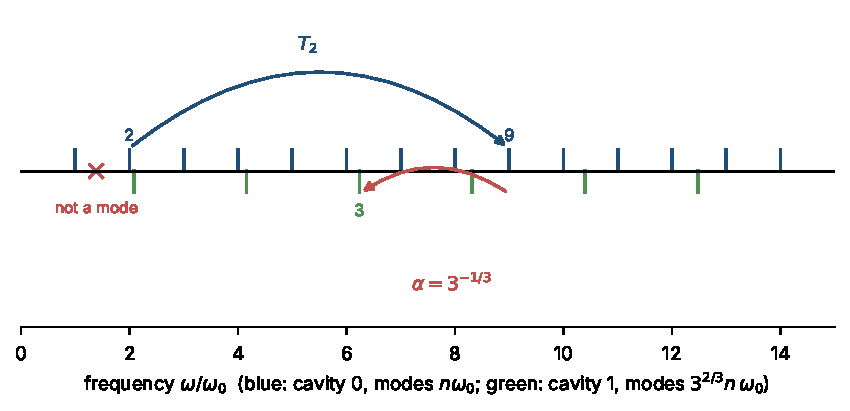
\includegraphics[width=.92\textwidth]{figures/fig_two_cavity_carry.pdf}\caption{Two periodic cavities, $\alpha=3^{-1/3}$. The carry cannot act on mode~$2$ of cavity~0 (cross: not a mode of cavity~1) but acts on mode~$9=T_2(2)$, landing on mode~$3$ of cavity~1.}\label{fig:two}\end{figure}
\begin{remark}[What this is, and is not]
In these coordinates the carry is the \emph{rational} map $n\mapsto c_in$; all irrationality sits in the ratio of the cavity sizes. The construction is therefore a precise statement about spectral commensurability of separately specified cavities, equivalent to ordinary rational-index bookkeeping, together with the observation that UNNS steps change the divisibility needed for the carry. It is not a mode-conversion mechanism: the two cavities are not coupled, and no energy transfer, boundary matching or overlap integral is defined. The fields on the two sides are related by a dilation, not by physical propagation.
\end{remark}

%% ----------------------------------------------------------------
\section{Carries inside one cavity: lattice similarities}\label{sec:sim}
A torsion carry inside a single cavity would have to map the mode lattice $\Z^D$ to itself. Maxwell is invariant under rotations $R$ and dilations, so the natural field map is
\[
\bE'(\mathbf r,t)=R\,\bE(\alpha R^{-1}\mathbf r,\alpha t),\qquad \bB'\ \text{likewise},
\]
which sends wave vector $\mathbf k$ to $\alpha R\mathbf k$ and keeps the polarization transported by $R$. It maps lattice modes to lattice modes iff $M=\alpha R$ preserves $\Q^D$-rationality of the lattice, i.e.\ $M\in GL_D(\Q)$ with $M^{\mathsf T}M=\alpha^2I$.

\begin{theorem}[Lattice similarities]\label{thm:sim}
Let $\lambda>0$. A matrix $M\in GL_D(\Q)$ with $M^{\mathsf T}M=\lambda^2I$ exists only if $\lambda^2\in\Q$, and:
(a) for $D$ odd, only if $\lambda\in\Q$;
(b) for $D=2$, iff $\lambda^2$ is a sum of two rational squares $a^2+b^2$, with $M=\left(\begin{smallmatrix}a&-b\\b&a\end{smallmatrix}\right)$ up to a reflection;
(c) for $D=4$, for every $\lambda^2\in\Q_{>0}$.
\end{theorem}
\begin{proof}
$\lambda^2=(M^{\mathsf T}M)_{11}\in\Q$. Taking determinants, $(\det M)^2=\lambda^{2D}$, so $\lambda^D\in\Q$; for $D$ odd $\lambda=\lambda^D/(\lambda^2)^{(D-1)/2}\in\Q$, giving (a). For $D=2$ the two rows are orthogonal of equal length, hence $(a,b),(-b,a)$ up to the sign of the second row, and $\lambda^2=a^2+b^2$; conversely this matrix works. For (c) write $\lambda^2=u/v$ in integers; Lagrange gives a quaternion $q\in\Z^4$ of norm $uv$, left multiplication by $q$ has $M_q^{\mathsf T}M_q=uv\,I$, and $M=M_q/v$ has $M^{\mathsf T}M=(u/v)I$.
\end{proof}
(Brute-force check of the integer case: for $\sigma\le40$ an integer matrix with $M^{\mathsf T}M=\sigma I$ exists in $D=2$ iff $\sigma$ is a sum of two squares and in $D=3$ iff $\sigma$ is a perfect square; V9.)

\begin{corollary}\label{cor:3d}
On the periodic $3$-torus no map $\bE'=R\bE(\alpha R^{-1}\cdot,\alpha\,\cdot)$ with $\alpha\notin\Q$ sends the mode lattice to itself. The spectral relations between direction classes of Theorem~\ref{thm:cls} (frequency ratios $\sqrt{\sigma\sigma'}/\gcd$) are real, but they are not induced by a field-level symmetry of the cavity; a carry between such classes must connect different cavities (Section~\ref{sec:cav}) or involve additional structure.
\end{corollary}

\subsection{The planar torus: Gaussian carries}
Consider fields periodic in $(x,y)$ with side $L$ and wave vectors in the plane, $m\in\Z^2$, $\omega=\omega_0|m|$ (TM$_z$ and TE$_z$ families). By Theorem~\ref{thm:sim}(b) the carry $\alpha=\sqrt\sigma$ is a field-level symmetry iff $\sigma=a^2+b^2$, and it is multiplication by the Gaussian integer $\gamma=a+ib$ on $m\in\Z[i]$.

\begin{proposition}[The $\sqrt2$ layers]\label{prop:gauss}
Let $\gamma=1+i$ and $\alpha=\sqrt2$, with $R$ the rotation by $45^\circ$. The map $m\mapsto\gamma m$ is the carry: it takes class $\sigma=1$ to $\sigma=2$ with the layer index $n$ unchanged ($c_0=1$) and class $\sigma=2$ to $\sigma=1$ with $n\mapsto2n$ ($c_1=2$), exactly as in~\cite{TC}. The inverse carry $\alpha=1/\sqrt2$ is admissible at $m$ iff $\gamma\mid m$, i.e.\ iff $m_x+m_y$ is even; on layer $0$ this means $n$ even ($c_0=\tfrac12$) and on layer $1$ it always holds ($c_1=1$), again as in~\cite{TC}.
\end{proposition}
\begin{proof}
For $m=g\,u$, $|\gamma m|^2=2|m|^2$, which gives $|m|=n\sqrt\sigma\mapsto n\sqrt{2\sigma}$ and the stated layer maps: from $\sigma=1$, $|\gamma m|=n\sqrt2$ (layer~1, index $n$); from $\sigma=2$, $|\gamma m|=2n$ (layer~0, index $2n$). For the inverse, $\gamma\mid m$ iff $m_x+m_y\equiv0\pmod2$ (since $m_x+m_y=\mathrm{Re}\,m+\mathrm{Im}\,m$, and $(1+i)(a+ib)=(a-b)+i(a+b)$); and $m_x+m_y\equiv m_x^2+m_y^2=n^2\sigma\pmod 2$, which is $n\bmod2$ for $\sigma=1$ and $0$ for $\sigma=2$.
\end{proof}
(Checked on all $888$ modes with $|m_{x,y}|\le60$ lying in the classes $\sigma\in\{1,2\}$; V11. The field map itself is verified symbolically: the TM mode $m=(3,0)$ goes to $m=(3,3)$ and then to $(0,6)$, with exact Maxwell residuals zero and periodicity in $x$ and $y$; V10.)

\begin{figure}[ht]\centering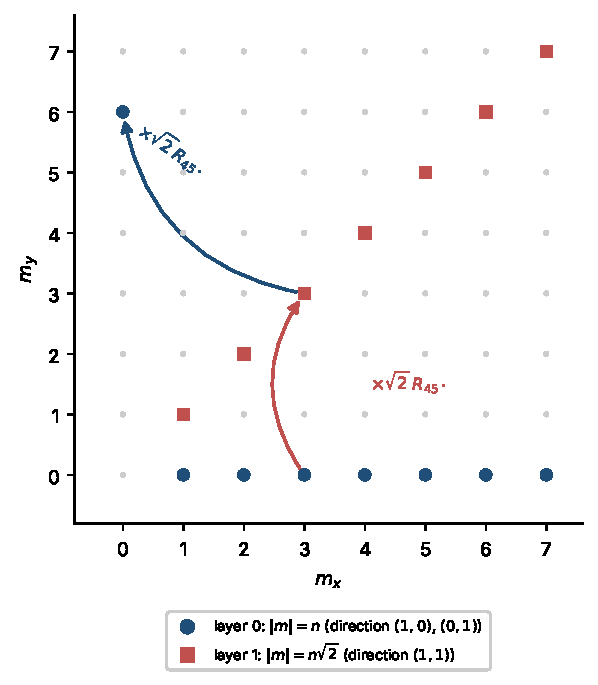
\includegraphics[width=.5\textwidth]{figures/fig_similarity_carry.pdf}\caption{The $\sqrt2$ carry on the square torus: $m=(3,0)\to(3,3)\to(0,6)$.}\end{figure}

\begin{remark}
In the planar torus the carry is therefore a genuine Maxwell symmetry map between direction classes, with no conditions for $\alpha=\sqrt2$, and with a divisibility condition (in $\Z[i]$, strictly arithmetic) for $\alpha=1/\sqrt2$. The realized classes in the plane are the squarefree $\sigma$ whose odd prime factors are $\equiv1\pmod4$; these are closed under the carry products. The planar picture contains the two-layer $\sqrt2$ system of~\cite{TC} as an exact sub-system, but it also has a feature absent from the abstract layers: for $\sigma$ not a sum of two squares (for example $\sqrt3$) there is no intra-cavity carry at all.
\end{remark}
\begin{remark}[Conducting walls]
The wall conditions of a box are not invariant under a $45^\circ$ rotation, so the similarity carry is not expected to survive in the conducting box, where only isotropic dilations (Proposition~\ref{prop:box}) remain. We have not checked this and record it as a target for v002.
\end{remark}

%% ----------------------------------------------------------------
\section{What is and is not new}
\begin{itemize}
\item \textbf{Inherited (label-level), no new physics.} The content/direction decomposition, the ray structure, the $\gcd$ reduction, the layered spectra of Section~\ref{sec:cav} and the enabling example are statements about integer and rational bookkeeping of mode labels, and a spectral theorist reaches them from commensurability alone. The torus classes of Theorem~\ref{thm:cls} are classical number theory applied to the spectrum $|m|$.
\item \textbf{Field-level, but already implied by Maxwell's dilation and rotation symmetries.} Theorem~\ref{thm:tr}, Propositions~\ref{prop:box} and~\ref{prop:hist}. The one non-obvious conclusion is negative: the field retains no history, so any invariant that distinguishes histories must live in the labels.
\item \textbf{Field-level, structural.} Theorem~\ref{thm:sim} and Corollary~\ref{cor:3d} classify which torsion carries are Maxwell symmetries of a single cavity, depending on the dimension of the lattice. This is a restriction on the carry mechanism imposed by electromagnetic geometry, not an arithmetic consequence of $M\perp N$.
\end{itemize}
\textbf{Not claimed.} No mode-conversion, coupling or energy-transfer mechanism; no statement about dispersive or lossy media; no comparison with the FUG-I history invariants beyond Proposition~\ref{prop:gcd}, which is elementary. The unrestricted nesting grammar is the one of~\cite{MX}; the torsion carries are an added generator, not selected by $M\perp N$.

\section{Directions for v002}
(a) Complete ancestry and reconvergence of $T_N$-histories on the rays of Proposition~\ref{prop:cd}, compared with the FUG-I history baseline once its records are placed alongside. (b) The planar torus with several carries ($\sqrt2$ and $\sqrt5$): coupled transition system on $\Z[i]$ with $T_N$ acting on the integer content; whether the layer structure gains connectivity or branching not present on the abstract layers. (c) Conducting boxes and cylinders: boundary-condition obstruction of the similarity carry. (d) Material dispersion: where dilation symmetry breaks and what survives.

%% ----------------------------------------------------------------
\begin{thebibliography}{9}\small\raggedright
\bibitem{AT} UNNS Research Collective, \emph{Algebraic and Topological Extensions of the UNNS Generative Law}, v1.1, November 2026.
\bibitem{TC} UNNS Research Collective, \emph{Torsion-Class Carry Dynamics and Generalized UNNS Admissibility}, v1.0, November 2026.
\bibitem{MX} UNNS Research Collective, \emph{Maxwell vacuum-field nesting investigation} (\texttt{investigations/MAXWELL}: \texttt{README.md}, \texttt{theory/SCALE\_TRANSPORT.md}, \texttt{results/EXAMPLES.md}).
\bibitem{J} J. D. Jackson, \emph{Classical Electrodynamics}, 3rd ed., Wiley, 1999 (periodic and cavity modes, scale and rotation symmetry).
\bibitem{G} E. Grosswald, \emph{Representations of Integers as Sums of Squares}, Springer, 1985 (Legendre's three-square theorem).
\bibitem{HW} G. H. Hardy and E. M. Wright, \emph{An Introduction to the Theory of Numbers}, 6th ed., Oxford, 2008 (sums of two and four squares).
\end{thebibliography}
\end{document}
